\quad 1.\quad В ходе работы с виртуальной машиной возникла необходимость перенести её с одного своего устройства на другое.
\newline Для этого открываем Virtual Box, нажимаем правой кнопкой мыши по своей виртуальной машине и выбираем пункт клонировать. В появившемся окне указываем имя нового клона и его путь, по которому он будет сохранён. Так же в графе «Политика MAC-адреса» выбираем вариант: «Сгенерировать новые MAC-адреса всех сетевых адаптеров».

\begin{figure}[h]		
		\centering
		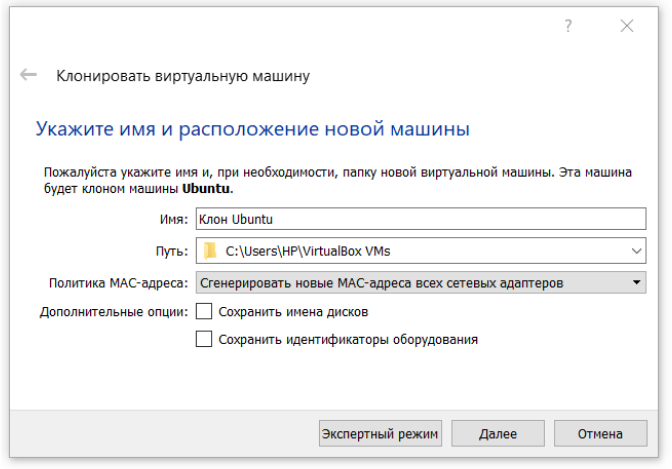
\includegraphics[width=0.6\linewidth]{VM/8.png}
\caption{Окно клонирования.}
\label{ris:image}
\end{figure}

\quad В следующем окне нужно было указать тип клонирования: полное или связное. При связном клонировании будет создана новая машина, использующая файлы виртуальных жёстких дисков клонируемой машины и нельзя перенести её на другой компьютер без переноса клонируемой. При полном клонировании, будет создана полная копия клонируемой виртуальной машины (включая все файлы виртуальных жёстких дисков). Поэтому выбиираем полное клонирование.

\quad В окне с указанием цели клонирования, указываем клонировать всё, чтобы новая машина не только отражала текущее состояние клонируемой машины, но и имела копии всех снимков её древа снимков.

\quad Далее нажимаем на кнопку «клонировать», после чего запускается процесс клонирования. По его завершению переносим новую машину на флэшку. Это можно сделать нажав в Virtual Box на клон правой кнопкой мыши и выбрать пункт «Переместить». Или просто зайти в папку, в которую был сохранён наш клон, и переместить его уже оттуда.

\quad Далее подсоединяем флэшку к другому компьютеру и переносим машину в папку Virtual Box. Открыв Virtual Box, нажиимаем вверху на кнопку «Машина» и выбрал пункт добавить. После чего находим свою машину и нажал кнопку «Открыть».

\begin{figure}[h]
		\centering
		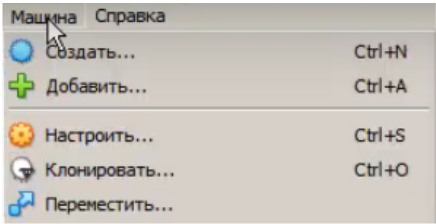
\includegraphics[width=0.4\linewidth]{VM/9.png}
\caption{Добавление виртуальной машины.}
\label{ris:image}
\end{figure}

\quad Виртуальная машина добавлена. Но зайдя в настройки, можно увидеть, что объём выделенной оперативной памяти составляет всего лишь 2 гигабайта, что слишком мало для работы с машиной. Так как наша машина находится в состоянии «Сохранена», мы не можем изменять её настройки. Поэтому нажимаем правой кнопкой мыши по перенесённому клону, и выбираем пункт «Сбросить сохранённое состояние». Сохранённое состояние, в отличие от снимка, это не остояние виртуальной машины на момент его создания, а актуальное состояние виртуальной машины, с которым работает пользователь, при каждом её запуске. Далее снова нажимаем правой кнопкой мыши по машине, выбираем пункт «Настроить…» и в «Системе» выделяем нужное количество памяти.

\begin{figure}[h]
		\centering
		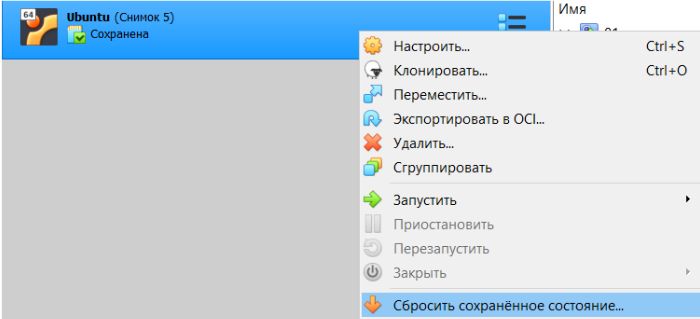
\includegraphics[width=0.75\linewidth]{VM/10.png}
\caption{Настройка памяти.}
\label{ris:image}
\end{figure}

\quad Далее заходим в «Носители» и выбираем свой жёсткий диск, так как иначе при запуске виртуальной машины мы бы ничего не увидели.

\begin{figure}[h]
		\centering
		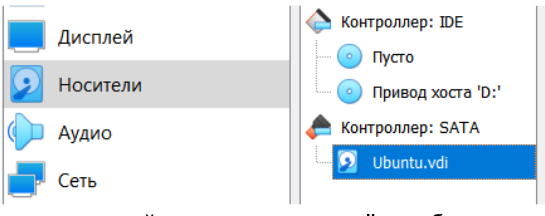
\includegraphics[width=0.5\linewidth]{VM/11.png}
\caption{Настройки. Носители.}
\label{ris:image}
\end{figure}

\quad Теперь клон виртуальной машины перемещён, добавлен на новый компьютер и с ним можно работать.

\quad Есть и альтернативный способ переноса виртуальной машины с одного устройства на другое, с помощью функций «Экспорт» и «Импорт».

